% In this section, we present our algorithm for computing the upper bound for a program $c$'s adaptivity
% $A(c)$ defined~\ref{def:trace_adapt} through static program analysis.
% This section presents the key definitions
% for the static analysis algorithm in Section~\ref{sec:algorithm-keys} before going into the detail of the algorithm,
% then shows the complete static analysis algorithm.
% \mg{
% In this section, we present our static program analysis for computing an upper bound on the adaptivity a program $c$
% }
In this section, we present our static program analysis for computing an upper bound on the 
reachability times on every location of an arbitrary program $c$, as we define in last section.
%
\subsection{A guide to the static program analysis framework}
In order to have the upper bound of the  reachability for every label of a program $c$, we design 
a path sensitive reachability bound analysis framework {\THESYSTEM}.
It can be divided as following steps: 
\begin{figure}
  \centering    
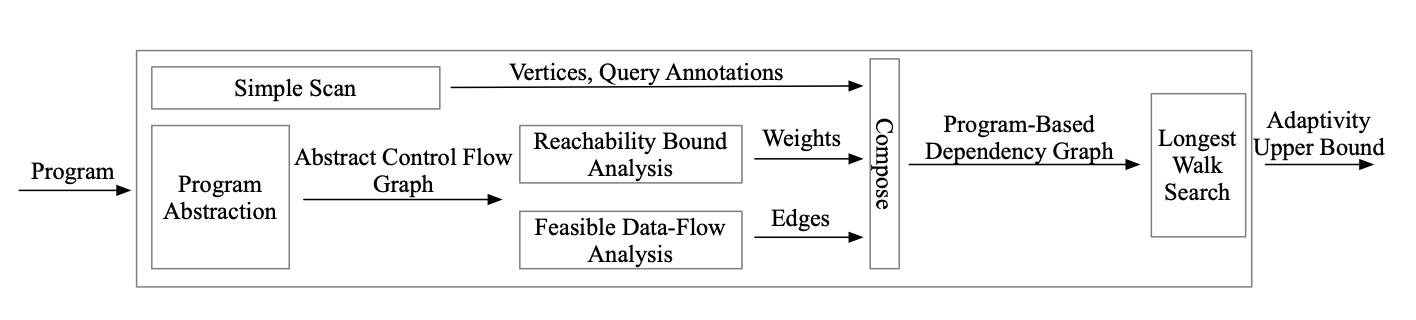
\includegraphics[width=1.0\columnwidth]{adapfun.png}
  \vspace{-0.3cm}
  \caption{The overview of {\THESYSTEM}}
  \label{fig:adaptfun}
  \vspace{-0.5cm}
\end{figure}
% \subsubsection{Graph Estimation}
%
%
\begin{enumerate}
\item  construct an abstract control flow graph based on $c$, by computing an abstract transition 
for every labeled command.
% see Section~\ref{sec:alg_vertexgen}
\item estimate an accurate upper bound for every while loop command of $c$.
% Vertices are the assigned variables with unique labels, which is extracted directly from the program, 
% Every vertex come with a weight, which tells the maximal times each vertex and edge can be visited in realistic execution. This weight is estimated by a reachability bound analysis on each vertex, See Section~\ref{sec:alg_weightgen}.
% \item Each edge also vertices considers both control flow and data flow, See
% Section~\ref{sec:alg_edgegen}
\item for every while loop, refine this while loop program into a path sensitive program.
\item perform the Outside-In and Inside-Out Algorithm on this path sensitive program, obtain 
accurate reachability bound for each path.
\item compute the reachability bound for every label in this program $c$ by summarizing overal the reachability bound for
each path and each loop.
% Finally, with all the ingredients ready, we construct the final approximated program-based dependency graph in Section~\ref{sec:alg_graphgen}
\end{enumerate}

% the algorithm  without extra static analysis technique.
% \\
% Overall, this program-based graph has a similar topology structure as 
% % the one
% % of 
% the Execution-Based Dependency Graph. It has the same
% vertices and query annotations, but approximated edges and weights. We call the graph generated by static analysis techniques, static analysis dedendency graph. 
% \item Then in the last phase in Section~\ref{sec:alg_adaptcompute}, $\THESYSTEM$
% % we compute the upper bound for adaptivity over this approximated graph:
% % , as an upper bound for
% % program's adaptivity
% computes the upper bound for adaptivity over this approximated graph.
% in the last phase of this algorithm in Section~\ref{sec:alg_adaptcompute}.
% \subsection{Adaptivity Based on Program Analysis in \THESYSTEM}
% In order to give a bound on the program's adaptivity, we first build a
% program-based data-dependency graph to {over-}approximate the
% trace-based dependency graph.  Then, we define a program-based
% adaptivity over this approximated graph, as an upper bound for
% $A(c)$.
% %
% \subsection{ $\THESYSTEM$ Analysis Algorithm}
% \subsection{Dependency Graph Estimation}
% \subsection{Vertices Estimationn}
% \label{sec:alg_vertexgen}
% The first component of every vertex in the static analysis dependency graph are actually identical as the  Execution-Based Dependency Graph, which are assigned variables in the program annotated with the unique label(line number). 
% These vertices are collected by statically scanning the program, like what we do for vertices of its Execution-Based Dependency Graph. 
% The vertices are defined formally as follows.

%   \highlight{
% \[
%     \progV^0(c) \triangleq \left\{ 
%   (x^l, w) \in \mathcal{LV} \times \mathcal{A}_{\lin}
%   ~ \middle\vert ~
%   x^l \in \lvar(c)
%   \right\}
%   \]
%   }
%   %
% where $\mathcal{A}_{\lin}$ is the set of arithmetic expressions over $\mathbb{N}$ and program's input variables. 
% The weight $w$ for every vertex will be computed in following step in Section~\ref{sec:alg_weightgen}.
% The static scanning of the programs also tells us whether one vertice(assigned variable) is assigned by a query request. We have similar definition when defining the Execution-Based Dependency Graph, 
% a set of pairs $\progF(c) \in \mathcal{P}(\mathcal{LV} \times \{0, 1\} )$ 
% % is the set of pairs 
% % The weight for each vertex in $\progV(c)$ is computed 
% mapping each $x^l \in \progV(c)$ to a flag, either $0$ or $1$, where $1$  means $x^{l}$ is a member of $ \qvar_{c}$, a set of those variables assigned with query requests, and $0$ means $x^{l}$ not in this set. It is defined formally below.

% \[\progF(c) =\left\{(x^l, n)  \in  \mathcal{LV} \times \{0, 1\} 
% ~ \middle\vert ~
% x^l \in \lvar_{c},
% n = 1 \iff x^l \in \qvar_{c} \land n = 0 \iff  x^l \not\in \qvar_{c} .
% \right\}\]
%

% \wq{To do: Add $\THESYSTEM$, a data flow analysis algorithm to scan the program and give a graph.}
% {\THESYSTEM} consists of three phases: 
% \begin{enumerate}
%     \item Generating an abstract control flow graph with each edge representing an abstract event transiting between two command labels. 
%     \item Computing the value bound invariant for each variable in the event and 
%     the event transition closure over the abstract control flow graph,
%     we get the reachability bound for each labeled command.
%     \item Refining the abstract control flow graph with data-flow, by performing the reaching definition analysis, we generate a weighted data control flow graph.
%     \item An algorithm to find the appropriate path in the weighted data control flow graph
% \end{enumerate}

% \begin{enumerate}
%     \item An algorithm to generate a precise data control flow graph
%     \item An algorithm to perform a Reachability number analysis to calculate the weight of each node in the graph generated in phase 1.
%     \item An algorithm to find the appropriate path in the weighted data control flow graph
% \end{enumerate}

% \subsection{Edge and Weight Estimation}
% \label{sec:alg_weightedgegen}

% Since the edges of the execution-based graph of a program relies on the dependency relation, which handles both control flow and data flow, as an over-approximation of this graph, the edges of our static anlaysis dependency graph also covers these two kind of flows. We develop a feasible data flow relation to catch these two flows, in Section~\ref{sec:alg_edgegen}.


% The weight of every vertice in the execution-based graph is built on all possible execution traces.
% In order to over-approximate the weight statically but still tightly, we present a symbolic reachability bound analysis for estimation of the weight of each vertice(label) in Section~\ref{sec:alg_weightgen},
% in spirit of some reachablility bound techiniques.


% The edges and weight estimation are both performed on basis of an abstract control flow graph of the program, we first show how to generate this abstract execution control flow graph before the introduction of  the edge and weight estimation.  

% This analysis first 
%  generate an abstract control flow graph
%  over all program labels, 
% in order to analyzing the data flow relations through variables assigned in every labeled command,
% and the reaching time of each variable.
% Then, it refines this control flow graph 
% % into a weighted data-dependency graph, 
% and generate the Program-Based Dependency Graph,
% through the data flow and reaching bound analysis results.
% In the last step, it finds the longest finite walk in this weighted data control flow graph w.r.t. the query variables,
% and return the number of query vertices traversed alongside.
% % \wq{To do: Add $\THESYSTEM$, a data flow analysis algorithm to scan the program and give a graph.}
% To be more specific, {\THESYSTEM} consists of five phases as follows,
% \\
% % \jl{Better to have a graph or picture of overview of the algorithm}
% \todo{graph}
% \todo{pass again}
% This analysis
% \begin{enumerate}
%     % \item Generating 
%     \item first generate 
%     an abstract control flow graph
%     %  over all labels,
%     (remove?? with program's labels as vertices and abstract transitions as edges)
%     in Section~\ref{sec:abscfg},
%     % used to analyze 
%     for analyzing the weight of every vertex in $\progV(c)$ and edges between every vertex in $\progV(c)$ in the next two steps;
%     %  \ref{sec:alg_weightgen} and 
%     % \ref{sec:alg_edgegen}.

%     % which are used as program's control locations,
%     %
%     \item then use the abstract control flow graph generated above, 
%     compute the weight of every vertex in $\progV(c)$ by computing a symbolic reachability bound for each label in Section~\ref{sec:alg_weightgen},
%     % \\
%     \item and then use the same graph again to estimate the edges between every vertex in $\progV(c)$ by computing the feasible data flow relation between every labeled variables in Section~\ref{sec:alg_edgegen}.
  
% \end{enumerate}

\subsection{Abstract Execution Control Flow graph}
\label{sec:abscfg}
The execution-based reachability bound of every label
%  in the execution-based graph 
is built on  execution traces.
In order to over-approximate the weight statically but still tightly, we present a symbolic reachability bound analysis for estimation of the weight of each vertice(label) in Section~\ref{sec:alg_weightgen},
in spirit of some reachablility bound techiniques.

This estimation is performed on basis of an abstract control flow graph of the program, we first show how to generate this abstract execution control flow graph before the introduction of  the edge and weight estimation.  

% In an 
%  % a program $c$ 
%  abstract control flow graph for a program $c$, $\absG(c)$, 
%  every 
%  vertex corresponds to the unique
%  label.
%  Specifically,
%  The edge is directed, 
%   representing an abstract transition 
%   between two control locations uniquely decided by the labels.   
%    (We refer control location and the label to the same thing). The abstract transition is of the form of a set of difference constraints for variables, built from the abstract execution trace of the program. For instance, the edge $(l_1, dc, l_2)$ from $l_1$ to $l_2$,
%   represents an abstract transition 
%   between two control locations with a set of difference constraints on it.
%  In this transition, the  command labeled with the second location $l_2$, 
%   will be executed after execution of the command with label $l_1$,
%  %  The abstract transition contains a set of difference constraints for variables, 
%  with the difference constraints generated by abstracting the command of the first label. Difference constraints is a constraint on difference between variables and constants, which will be formally introduced when we discuss experssion abstraction.
%  \wq{The edge in the abstract control flow graph comes from the abstract execution trace of the program. The abstract execution trace, an abstract representation of the execution, consists of a list of abstract transitions. Then, every abstract transition in the abstrction execution trace corresponds to an edge in the abstract control flow graph. In aonther word, the edge $(l_1, dc, l_2)$ in the abstract control flow graph, represents an abstract transition 
%   from $l_1$ to $l_2$, with a set of difference constraints $dc$. Also notice, the difference constraints generated during the abstract transition appears in the edge as annotation.}

%  % over program's abstract execution 

%  Overall, the key point of the abstract excution control flow graph is the construction of the abstract execution trace of a program, which relies on a program abstraction procedure in following steps:

%  \begin{enumerate}
%  \item  Computing the abstract expression for every assignment command in the program.
%  \item Computing the abstract event for every labeled command in the program. Intuitively, this abstract event aims 
%  to approximate the event in program's execution trace.
%  \item Constructing the abstract execution trace for a program.
%  \end{enumerate}  

We discuss the vertices and edge of the
abstract control flow graph for a program $c$, $\absG(c)$.

Every 
vertex corresponds to the unique
label.
Specifically,
the vertices of this graph is the set of $c$'s labels with an exit label $l_{ex}$, 
\[ 
  \absV(c) = labels(c)\cup\{l_{ex}\}
  \]
%  corresponding to a label command in the program.

% \wq{
  The edge in the abstract control flow graph comes from the abstract execution trace of the program. 
  The abstract execution trace, an abstract representation of the execution, consists of a list of abstract transitions. 
  Then, every abstract transition in the abstraction execution trace corresponds to an edge in the abstract control flow graph. In another word, the edge $(l_1, dc, l_2)$ in the abstract control flow graph, represents an abstract transition 
 from $l_1$ to $l_2$, with a set of difference constraints $dc$. 
 Also notice, the difference constraints generated during the abstract transition appears in the edge as annotation.
%  }

% over program's abstract execution 


% \wq{
  Overall, the vertices can be easily collected and the key point of construction of the abstract execution control flow graph for a program is the abstract execution trace, 
  which relies on the abstraction of expression and abstract transition (we also call it abstract event), we will discuss in the following section.
   To make it easy to understand, abstract control flow graph is a control flow graph, with difference constraints on every edge.
  % }  

%
\paragraph*{Expression Abstraction}

The expression assigned to the variable on the left hand of the assignment command is abstracted to an abstract value: (adopted from the expression abstraction method in paper \cite{sinn2017complexity}). The abstract value is expressed in the form of Difference constraint, denotated as $DC : \mathcal{VAR} \cup \constdom \to \mathcal{\mathcal{VAR} \times (\mathcal{VAR} \cup \constdom) } \times (\mathbb{Z} \cup \{\infty\})$.  $\constdom$ is called the Symbolic Constant defined as $\constdom \triangleq \mathbb{N} \cup \inpvar \cup \{\max{(\dbdom)}\} $, which consists of 
natural numbers $\mathbb{N}$,
the program's input variables $\inpvar$  
and a constant value $Q_m$ for estimating the upper bound of variables which are
assigned by queries. 

Give an instance of difference constraint used here,
$DC(\mathcal{VAR}  \cup \constdom) \cup \{\top\}$ represents all the difference constraints over 
variable and symbolic constants. 
% The difference constraint $DC$ over $\mathcal{VAR} \cup \constdom$ 
It is a set of the inequality of form $x \leq y + v$ where $x \in \mathcal{VAR} $, 
$y \in \mathcal{VAR}  \cup \constdom$ and $v \in \mathbb{Z}$. 
This difference constraint is defined in the same way as
\cite{sinn2017complexity}. For concise, we use $\dcdom^{\top}$ to represent the $DC(\mathcal{VAR}  \cup \constdom) \cup \{\top\}$ .


We show the expression abstraction $\absexpr : \expr \to \mathcal{VAR} \to DC(\mathcal{VAR}  \cup \constdom) \cup \{\top\} $ below.

% We introduce the following notations and operations first
% % an expression abstraction method based on the expression abstraction in paper \cite{sinn2017complexity}.
% \\
% % is enriched into $\constdom \triangleq \mathbb{N} \cup \inpvar \cup \{\max{(\dbdom)}\} $.
% T
% \\

% represents the set of inequality over all $\mathcal{VAR}  \cup \constdom$. 

% The symbolic constant is enriched into $\constdom \triangleq \mathbb{N} \cup \inpvar \cup \{\max{(\dbdom)}\} $.
% It consists of 
% natural number $\mathbb{N}$,
% the symbolic constants $\inpvar$ (i.e., the set of the program's input variables), 
% and a constant value $Q_m$ for estimating the upper bound of variables which are
% assigned by queries.
% \\
% The symbolic constant is enriched into $\constdom \triangleq \mathbb{N} \cup \inpvar \cup \{\max{(\dbdom)}\} $.
% \\

% % $ \absdom: \mathcal{P}(DC(\mathcal{VAR}  \cup \constdom) \cup \{\top \})$:
% \\
% $\constdom: \mathbb{N} \cup \inpvar \cup \{\max{(\dbdom)}\} $ 
% The  constant 
% \\
% % $DC(\mathcal{VAR}  \cup \constdom)$ represents the set of inequality over all $\mathcal{VAR}  \cup \constdom$.
% \\

% \[
%   \begin{array}{ll} 
%     \absexpr(y + c, x)  = x' \leq y + c  & c \in \mathbb{N} \land y \in (VAR \cup \constdom) \\
%     \absexpr(y - c, x)  = x' \leq y - c  & c \in \mathbb{N} \land y \in (VAR \cup \constdom) \\
%     \absexpr(v, x)  = x' \leq v + 0  & v \in (VAR \cup \constdom) \\
%     \absexpr(\aexpr, x) = x' \leq 0 + \infty   & \aexpr \text{ doesn't have any of the forms as above} \\
%     \absexpr(\qexpr, x)  = x' \leq 0 + Q_m & \qexpr \text{ is a query expression}  \\
%     \absexpr(\bexpr, x) = x' \leq 0 + 1   & \bexpr \text{ is a boolean expression} \\
%   \end{array}
%   \]
  \[
    \begin{array}{ll} 
      \absexpr(x - v, x)  = x' \leq x - v  & x \in \grdvar \land v \in \mathbb{N} \\
      \absexpr(y + v, x)  = x' \leq y + v  & x \in \grdvar \land v \in \mathbb{Z} \land y \in (\grdvar \cup \constdom) \\
      \absexpr(v, x)  = x' \leq v + 0  & x \in \grdvar \land v \in (\grdvar \cup \constdom) \\
      \absexpr(y + v, x)  = x' \leq y + v & \\
      \grdvar = \grdvar \cup \{y\} & x \in \grdvar \land v \in \mathbb{Z} \land y \notin (\grdvar \cup \constdom)  \\
      \absexpr(\qexpr, x)  = x' \leq 0 + Q_m & x \in \grdvar \land \qexpr \text{ is a query expression}  \\
      \absexpr(\bexpr, x) = x' \leq 0 + 1   & x \in \grdvar \land \bexpr \text{ is a boolean expression} \\
      \absexpr(\expr, x) = x' \leq \infty  &  x \in \grdvar \land \expr \text{ doesn't have any of the forms as above} \\
      \absexpr(\expr, x) = \top  &  x \notin \grdvar \\
    \end{array}
    \]
  
  % \wq{ 
    $\grdvar$ is the set of variables used in the guard expression of every while command in the program $c$. 
  % }. 
  In the case 4, if a variable $x$, belonging to the set 
  $\grdvar$ is updated by a variable $y$, which isn't in this set, 
  we add $y$ into the set $\grdvar$ and repeat 
  above procedure  until $\grdvar$ and $\absexpr(\expr, x)$ is stabilized. 
  % \wq{I do not understand this sentence:-(}
  \\
Specifically 
% understanding the intuition, 
we handle a 
% simplified 
normalized guard expression ($ x > 0$ for $x^l \in \lvar_c$)
 in $\ewhile$, and 
%  \wq{I do not understand this sentence:-(}
%  .
% \\
% The counter variables only increase, decrease or reset by expression in the form of arithmetic minus and plus (able to extend to max and min.)
the counter variables only increase, decrease or reset by 
% expression in the form of 
simple arithmetic expression (mainly multiplication, division, minus and plus (able to extend to max and min)). 
This is the same as in paper \cite{sinn2017complexity}. 
\\
For more complex expression assignments, where the counter reset, or calculated from $\elog$, 
multiplication or division, and expressions involving multiple variables, the constraint is approximated as reset of $\infty$.
\\
% This simplification \wq{which part we simplify here?} 
This approximation strategy
doesn't affect our analysis results in our examples. It is easy to extend the normalized expression 
into more complex forms as in \cite{sinn2017complexity}, as well as the 
counter variable manipulation with more advanced expressions.
% \\ 
% The boolean expression in the guard of $\ewhile$ command is normalized into form of $ x > 0$ where $x^l \in \lvar_c$ for some $l$.


\paragraph{Program Event Abstraction}
We show the abstract event definition, which is generated when computing its abstract execution trace.

\begin{defn}[Abstract Event]
  \label{def:abs_event}
  Abstract Event: 
  $\absevent \in $
  $\ldom \times \dcdom^{\top} \times \ldom$
  is a 
  % pair of abstract initial state and final state.
  triple where the first and third components are labels,
  second component is a constraint from $\dcdom^{\top}$.
  % the thrid % computed from program's abstract final and initial state, $\absfinal(c)$ and $\absinit(c)$ with formal definition, and algorithm detail in Appendix.
  %  the constraint and the third corresponds to a final state.
  \end{defn}
  Specifically, in an abstract event, 
  the first label correspond to an initial state, and 
  the second label and the constraint correspond to an abstract final state.
 The abstract initial state is a label from $\ldom$.
The abstract final state is a pair from $\ldom \times \dcdom^{\top}$,  
where first component is a label from $\ldom$ and the second component is a constraint from $\dcdom^{\top}$.
%

%
Given a program $c$, its abstract initial state,
and the set of its abstract final state is computed as follows,
%
\[
  \begin{array}{ll}
    \absinit(\clabel{\assign{x}{\expr}}{}^l)  & = l  \\
    \absinit(\clabel{\assign{x}{\expr}}{}^l)  & = l \\
    \absinit(\clabel{\eskip}^{l})  & = l \\
    \absinit(\eif [b]^l \ethen c_1 \eelse c_2)  & = l \\
    \absinit(\ewhile [b]^l \edo c)  & = l \\
    \absinit(c_1 ; c_2)  & = \absinit(c_1) \\
 \end{array}
 \]
%
Final State Abstraction: 
$\absfinal: \cdom \to \mathcal{P}(\ldom \times \dcdom^{\top})$,
computes the set of Abstract Final State for the command. 
 \[
  \begin{array}{ll}
    \absfinal(\clabel{\assign{x}{\expr}}{}^l)  & = \{(l, \absexpr\eapp (\expr, x))\}  \\
     \absfinal(\clabel{\assign{x}{\query(\qexpr)}}{}^l)  & = \{
      (l, x' \leq 0 + Q_m )\}  \\
     \absfinal(\clabel{\eskip}^{l})  
     & = \{(l, \top)\} \\
     \absfinal(\eif [b]^l \ethen c_1 \eelse c_2)  & = \absfinal(c_1) \cup \absfinal(c_2) \\
     \absfinal(\ewhile [b]^l \edo c)  & = \{(l, \top)\} \\
     \absfinal(c_1 ; c_2)  & =  \absfinal(c_2) \\
 \end{array}
 \]
 %
 \paragraph{Abstract Execution Trace}
 Now, we  extract the abstract execution trace  $\absflow(c)$ for a program, which computes the Abstract Execution Trace for program $c$, as a set of the abstract events $\absevent$.
 %
 \begin{defn}[Abstract Execution Trace]
 \label{def:abs_trace}
  $\absflow \in \cdom \to \mathcal{P}( \ldom \times DC(\mathcal{VAR}  \cup \constdom) \cup \{\top\}) \times \ldom )$
  \end{defn}
 %

 
  We now show how to compute the abstract execution trace. 
  For simplicity, we use $\mathcal{P}(\absevent)$ represent the power set of all abstract events, and we have $\absflow(c) \in \mathcal{P}(\absevent)$.
 We first append a skip command with 
%  a symbolic label $l_e$, i.e., $\clabel{\eskip}^{l_e}$ at the end of the program $c$, and compute the $\absflow(c) = \absflow'(c')$ for $c'$, where $c' = c;\clabel{\eskip}^{l_e}$ as follows,
the exist label $l_{ex}$, i.e., $\clabel{\eskip}^{l_{ex}}$ at the end of the program $c$, 
and compute the $\absflow(c) = \absflow'(c')$ for $c'$, where $c' = c;\clabel{\eskip}^{l_{ex}}$ as follows,
 %
 {\footnotesize
 \[
   \begin{array}{ll}
      \absflow'(\clabel{\assign{x}{\expr}}{}^l)  & = \emptyset  \\
      \absflow'(\clabel{\assign{x}{\query(\qexpr)}}{}^l)  & = \emptyset  \\
      \absflow'([\eskip]^{l})  & = \emptyset \\
      \absflow'(\eif [b]^l \ethen c_t \eelse c_f)  & =  \absflow'(c_t) \cup \absflow'(c_f)
      %   \\ & \quad 
        \cup \{(l, \top,  \absinit(c_t) ) ,  (l, \top, \absinit(c_f)) \} \\
       \absflow'(\ewhile [b]^l \edo c_w)  & =  \absflow'(c_w) \cup \{(l, \top, \absinit(c_w)) \} 
      %  \\ & \quad 
       \cup \{(l', dc, l)| (l', dc) \in \absfinal(c_w) \} \\
       \absflow'(c_1 ; c_2)  & = \absflow'(c_1) \cup  \absflow'(c_2) 
      %  \\ & \quad 
       \cup \{ (l, dc, \absinit(c_2)) | (l, dc) \in \absfinal(c_1) \} \\
   \end{array}
   \]
   }

   Notice $\absflow'([x := \expr]^{l})$, $\absflow'([x := \query(\qexpr)]^{l})$ and $\absflow'([\eskip]^{l})$ are all empty set. 
   For every event $\event$ with label $l$ in an execution trace $\trace$ of program $c$, 
   there is an abstract event in program's abstract execution trace of form $(l, \_, \_)$.  
   We also show the soundness of the abstract execution trace in Appendix.
  %  which says 
  %  \wq{...}
   \begin{lem}[Soundness of the Abstract Execution Trace]
     \label{lem:abscfg_sound}
   Given a program ${c}$, we have:
   %
   \[
     \begin{array}{l}
       \forall \vtrace_0, \trace \in \mathcal{T} ,  \event = (\_, l, \_) \in \eventset \st
   \config{{c}, \trace_0} \to^{*} \config{\eskip, \trace_0 \tracecat \vtrace} 
   \land \event \in \trace 
   \\
   \qquad \implies \exists \absevent = (l, \_, \_) \in (\ldom\times \dcdom^{\top} \times \ldom) \st 
   \absevent \in \absflow(c)
   \end{array}
   \]
   \end{lem}
%    This lemma is proved formally in Appendix~\ref{apdx:reachability_soundness}.
% For every event $\event$ with label $l$ in an execution trace $\trace$ of program $c$, 
% there is an abstract event in program's abstract execution trace of form $(l, \_, \_)$. 
This lemma is proved formally in Lemma~\ref{lem:abscfg_sound} in Appendix~\ref{apdx:reachability_soundness}.
\\
For every labeled variable in program $c$, $x^l \in \lvar_c$, there is a unique abstract event in program's abstract execution trace $\absevent \in \absflow(c)$ of form $(l, \_, \_)$. 
\begin{lem}[Uniqueness of the Abstract Execution Trace]
  \label{lem:abscfg_unique}
Given a program ${c}$, we have:
%
\[
  \begin{array}{l}
    \forall \vtrace_0, \trace \in \mathcal{T} ,  \event = (\_, l, \_, \_) \in \eventset^{\asn} \st
\config{{c}, \trace_0} \to^{*} \config{\eskip, \trace_0 \tracecat \vtrace} 
\land \event \in \trace 
\\
\qquad \implies \exists! \absevent = (l, \_, \_) \in (\ldom\times \dcdom^{\top} \times \ldom) \st 
\absevent \in \absflow(c)
\end{array}
\]
\end{lem}
This lemma and proof is also 
formalized in Lemma~\ref{lem:absevent_unique} in Appendix~\ref{apdx:reachability_soundness}.

Then, we build the edge for $c$'s abstract control flow graph as follos,
\[
  \absE(c) = \{(l_1, dc, l_2) | (l_1, dc, l_2) \in \absflow(c)\}
  \]

% We have a pre-processing algorithm to go through the programs and returns the list of labels associating with a loop and whose visiting times need to be analyzed.
%


\paragraph{Abstract Control Flow Graph} 
With the vertices $\absV(c)$ and edges $\absE(c)$ ready, we construct the abstract control flow graph, formally 
% Through a program $c$'s abstract execution trace, its abstract control flow graph is computed 
defined in 
Definition~\ref{def:abs_cfg}.
% Given program $c$ with its abstract control flow $\absflow(c)$, the Abstract Control Flow Graph:
% \\
\begin{defn}[Abstract Control Flow Graph]
\label{def:abs_cfg}
Given a program $c$, 
with its abstract control flow $\absflow(c)$
its abstract control flow graph $\absG(c) =(\absV(c), \absE(c), \absW(c))$ is defined as follows,
\\
% \highlight{
% :
%
% \\
$\absE(c) = \{(l_1, dc, l_2) | (l_1, dc, l_2) \in \absflow(c)\}$,
\\
$\absV(c) = labels(c)\cup\{l_{ex}\}$
\\
 $\absW(c) 
\triangleq \left\{ (l, w) \in \mathbb{L} \times EXPR(\constdom) \right\}$.
% }
% \\
% , where the weight of every label to be computed in the next step.
\end{defn}
% 
% The vertices $\absV(c)$ in this graph are program's labels with an exit label $l_{ex}$.
% Each directed 
%  edge $(l_1, dc, l_2)$ from $l_1$ to $l_2$,
%  represents an abstract transition 
%  between two control locations with a set of difference constraints on it.
% %  , i.e., the labels of two commands (we call the labels also control location and they refer to the same thing), 
% %  where 
% In this transition, the  command labeled with the second location $l_2$, 
%  will be executed after execution of the command with label $l_1$,
% %  The abstract transition contains a set of difference constraints for variables, 
% with the difference constraints generated by abstracting the command of the first label.
% % \\
% % It is easy to show for every $(l_1, dc, l_2) \in \absflow(c)$ such that $l_2 \neq l_e$, $(l_1, l_2) \in flow(c)$. The formal Lemma and proof can be found in Lemma~\ref{lem:flow_to_absflow} in Appendix~\ref{apdx:reachability_soundness}.
Notice we also define the $\absW(c)$ in this graph without giving an actual value.
This $\absW(c)$ is the set of weight for every 
% vertex 
label. The weight is a symbolic expression over the symbolic constant, 
which is the estimated upper bound on the number of visiting time for every control location
through the reachability bound analysis as follows.
%
% It is easy to show for every $(l_1, dc, l_2) \in \absflow(c)$ such that $l_2 \neq l_e$, $(l_1, l_2) \in flow(c)$. The formal Lemma and proof can be found in Lemma~\ref{lem:flow_to_absflow} in Appendix~\ref{apdx:reachability_soundness}.
%
\paragraph*{Example}
% Look at the two-round example again, its generated abstract control is shown as in Figure~\ref{fig:adapfun_tworound}(a).
% In this abstract control flow graph, every vertex is a label,
% corresponding to a label command in the program.
% Each directed 
% edge represents an abstract transition 
% between two control locations, 
% i.e., the labels of two commands (we call the labels also control location and they refer to the same thing), 
% where the second labeled command will be executed after execution of the command with first label.
% For example, the edge $0, a \leq 0, 1$ on the top, represents,
% from location $0$, the command 
% $\clabel{\assign{a}{0}}^0$ is executed with next continuation location $1$,
% where the 
% command $\clabel{\assign{j}{k}}^1$ will be executed next.
% The constraint $a \leq 0$ is generated by abstracting from the assignment command $\assign{a}{0}$,
% representing that value of $a$ is less than or equals to $0$ after 
% location $0$ before executing command at line $1$.
% %
% The same way for the rest edges' constructions.
%
Let us look at the two-round example, its generated abstract control flow graph is shown as in Figure~\ref{fig:abscfg_twoRounds}(b).
For example, the edge $(0, a \leq 0, 1)$ on the top, tells us the command 
$\clabel{\assign{a}{0}}^0$ is executed with next continuation location $1$,
where the 
command $\clabel{\assign{j}{k}}^1$ will be executed next.
The constraint $a \leq 0$ is a difference constraint, generated by abstracting from the assignment command $\assign{a}{0}$,
representing that value of $a$ is less than or equals to $0$ after 
location $0$ before executing command at line $1$. The difference constraint is an inequality relation between, the left-hand side of the inequality talks about the variable before the execution and the right-hand side ascribes those after the execution. 
Look at the $a < a+x $ on the edge $5$ to $2$, which describes the execution of the command at line $5$, which is an assignment $a = a+x$. The $a$ on the left side of $a < a+x$ represents the value of $a$ after the assignment, while the right-hand side $a$ stores the value before the assignment. 
Also, we have while loop, which is a circle $2 \to 4 \to 5 \to 2$ in Figure~\ref{fig:abscfg_twoRounds}(b). 
Please also look at the edge from $3$ to $4$, which talks about the query! The $x < Q_m$ describes the execution of a query request (the command at line 3), the query results stored in $x$ is bounded by $Q_m$. 
$Q_m$ is the maximal value for query requesting result from the database $DB$. $top$ means there is no assignment executed, for example, we have the difference constraint $\top$ on the edge $2$ to $6$, means at line $2$, there is no assignment (it is a testing guard $j>0$.) 
%
The same way for the rest edges' constructions.

%
\subsection{\highlight{Path Sensitive Reachability Bound Analysis}}
\label{sec:alg_rbgen}
%
% In order to estimate weight for every vertex in $\progV(c)$,
%  we first show how to compute the reachability bound for every label in $c$
%  % (i.e., every vertex in $\absV(c)$)
%  (i.e., the $\absW(c)$), 
%  then show how to compute the weight for every vertex in $\progV(c)$.
%  \\
%  Through the edges in $\absG(c)$, which correspond to $c$'s abstract transition between labels,

%  \wq{In order to estimate weight for every vertex in the static analysis dependency graph($\progV(c)$), we want to find out the upper bound on 
%  the number of times the labeled command (uniquely associated with a vertex in $\progV(c)$) may be executed when running the program.
%  This information can be obtained by computing the reachability bound for every vertice in the abstract control flow graph ($\absW(c)$), because
%  the vertices in the two graph share the same unique label, the line number. We can easily show that the reachability bound on one vertex of the actract control flow graph is also the upper bound for the corresponding vertex in the static analysis dependency graph, both vertices share the same unique line number.}



%  We perform the symbolic reachability bound anaysis on the abstract control flow graph, 
%  through the edges in $\absG(c)$, which correspond to $c$'s abstract transition between labels.
%  we infer the invariant for every variable, and compute the transition closure for every abstract transition. By solving the closure
%  with the invariants of variables involved in this closure for every transition, we compute
%  the symbolic reachability bound of every commands corresponding to this transition.
%  \\
%  Specifically in four steps, Variable Modification Tracking, Local Bounds Computation,
%  the symbolic reachability bound of every commands corresponding to this transition. Specifically, this analysis can be performed in four steps:
%   Variable Modification Tracking, Local Bounds Computation,
%  Invariant Inference and Closure Generation, and Reachability Bound Computation,
{In order to estimate weight for every vertex in the static analysis dependency graph($\progV(c)$), we want to find out the upper bound on 
the number of times the labeled command (uniquely associated with a vertex in $\progV(c)$) may be executed when running the program.
This information can be obtained by computing the reachability bound for every vertex in the abstract control flow graph ($\absW(c)$), because
the vertices in the two graph share the same unique label, the line number. We can easily show that the reachability bound on one vertex of the abstract control flow graph is also the upper bound for the corresponding vertex in the static analysis dependency graph, both vertices share the same unique line number.}


We perform the symbolic reachability bound analysis on the abstract control flow graph, 
through the edges in $\absG(c)$, which correspond to $c$'s abstract transition between labels.
We infer the invariant for every variable, and compute the transition closure for every abstract transition. By solving the closure
with the invariants of variables involved in this closure for every transition, we compute
the symbolic reachability bound of every commands corresponding to this transition. Specifically, this analysis can be performed in four steps:
 Variable Modification Tracking, Local Bounds Computation,
Invariant Inference and Closure Generation, and Reachability Bound Computation,
% 
% We present the details of invariant, closure generation, and reachability bound computation as follows.
with details as follows.
%
%
\paragraph*{Variable Modification Tracking}
Identify the abstract events where each variable is increased, decreased and reset:
\\
$\inc: \mathcal{VAR} \to \mathcal{P}(\absevent) $
the set of the abstract events where the variable increase.
\\
$\inc(x) = \{(\absevent, c) | \absevent = (l, l', x' \leq x + v)\}$
\\
$\reset: \mathcal{VAR} \to \mathcal{P}(\absevent) $
The set of the abstract events where the variable is reset.
\\
$\dec: \mathcal{VAR} \to \mathcal{P}(\absevent) $
The set of abstract events where the variable decrease.
% \\
% $\dec(x) = \{(\absevent, c) | \absevent = (l, l', x' \leq x - v)\}$
\\
$Incr(v) \triangleq \sum\limits_{(\absevent, c) \in \inc(v)}\{\absclr(\absevent) \times v\}$
%
\paragraph*{Local Bounds}
Given a program $c$ with its abstract control flow graph 
$\absG(c) = (\absV, \absE)$
\\
Local Bounds Computation:
$\locbound: \absevent \to \mathcal{VAR} \cup \constdom$.
%
\[ 
\begin{array}{ll}
  \locbound(\absevent) \triangleq 1 
  & \absevent \notin SCC(\absG(c))
  \\
  \locbound(\absevent) \triangleq (x, v) 
  & \absevent \in SCC(\absG(c)) \land \absevent \in \dec(x) \land  \absevent = (\_, \_ , x' \leq x - v) \\
  \locbound(\absevent) \triangleq (x, \max(\dec(x))) 
  & \absevent \in SCC(\absG(c)) \land 
  \absevent  \notin \bigcup_{x \in \mathcal{VAR}} \dec(x)
  \land \absevent \notin SCC(\absG(c) \setminus \dec(x)) 
\end{array}
  \]
  The first case is straightforward. Since variable's visiting time outside of any while loop is at most 1, we do not need to analyze the visiting times of every node in the graph from phase 1.
  The second and third step is guaranteed by the \emph{Discussion on Soundness} in Section 4 of \cite{sinn2017complexity}.
  Then soundness proof is in Lemma~\ref{lem:local_bound_sound} in Appendix~\ref{apdx:reachability_soundness}.
%
\paragraph*{Invariant Inference and Closure Generation }
Then, computing the bound invariants for variables and the transition closures for abstract events:
\\ 
$ \varinvar: \mathcal{VAR} \cup \constdom \to EXPR(\constdom)$
\\
$\absclr: \absevent \to EXPR(\constdom)$
\\
$EXPR(\constdom)$ is symbolic expression 
over $\constdom$, which is a subset of arithmetic expressions over $\mathbb{N}$ with input variables and $ $.
We use $\mathcal{A}_{\lin}$ denotes the arithmetic expression 
over the symbolic variables, (i.e., $\mathbb{N}$ with input variables and $ $).
Then, the symbolic invariant for each variable 
as well as the symbolic transition closure for each transition is calculated as follows:
\[ 
\begin{array}{lll}
  \varinvar(x) & \triangleq c & c \in \constdom \\
  \varinvar(x) & \triangleq Incr(v) + \max(\{\varinvar(a) + c | (t, a, c) \in \reset(x)\}) & c \notin \constdom
\end{array}
\]
%
\begin{defn}
  \label{def:transition_closure_base}
\[ 
\begin{array}{lll}
  \absclr(\absevent) 
  & \triangleq x / v & \\ 
  & \locbound(\absevent) = (x, v) \in \constdom \times \mathbb{N} & \\
  \absclr(\absevent) 
  & \triangleq (Incr(x) + 
  \sum\limits_{(\absevent', y, v') \in \reset(x)}
  \absclr(\absevent') \times \max(\varinvar(y) + v', 0) ) / v & \\
  & \locbound(\absevent) = (x, v) \land x \notin \constdom & 
\end{array}
  \]
\end{defn}
%
\paragraph*{Improved Variable Modification Tracking}
Instead of just identifying the abstract events where each variable is reset,
this improvement identifies the chain of the events where a given variable is reset by the 
variables of the abstract events through the chain.
\\
$\resetchain: \mathcal{VAR} \to \mathcal{P}(\mathcal{P}(\absevent)) $
The set of the chain of abstract events where the variable is reset through the chain.
% \\
% $Incr(v) \triangleq \sum\limits_{(\absevent, c) \in \inc(v)}\{\absclr(\absevent) \times v\}$
%
\paragraph*{Improved Invariant Inference and Closure Generation}
Then, computing the bound invariants for variables and the transition closures for abstract events:
\\ 
$ \varinvar: \mathcal{VAR} \cup \constdom \to \mathcal{A}_{\lin}$
\\
$\absclr: \absevent \to \mathcal{A}_{\lin}$
\\
Then, the symbolic invariant for each variable 
as well as the symbolic transition closure for each transition is calculated as follows:
\[ 
\begin{array}{lll}
  \varinvar(x) & \triangleq c & c \in \constdom \\
  \varinvar(x) & \triangleq Incr(v) + \max(\{\varinvar(a) + c | (t, a, c) \in \reset(x)\}) & c \notin \constdom
\end{array}
\]
%
\begin{defn}
  \label{def:transition_closure}
\[ 
\begin{array}{lll}
  \absclr(\absevent) 
  & \triangleq x / v & \\ 
  & \locbound(\absevent) = (x, v) \in \constdom \times \mathbb{N} & \\
  \absclr(\absevent) 
  & \triangleq \Big(
    \sum\limits_{y \in \{ y ~|~ 
    ch \in \resetchain(x), (l_1, x, y, v, l_2) \in ch \} } Incr(x) & \\
    & \quad + 
  \sum\limits_{ch \in \resetchain(x)}
  \big( \min\limits_{\absevent' \in ch}({\absclr(\absevent')}) \times 
  \max(\varinvar(y) + \sum\limits_{(l_1, x, y, v, l_2) \in ch } v, 0)\big) \Big) / v & \\
  & \locbound(\absevent) = (x, v) \land x \notin \constdom & 
\end{array}
  \]
\end{defn}
  %
% \paragraph*{Adding the Reachability Bounds for Every Vertex in the Data-Control Flow Graph}
% Updating the weight of every vertex in the $\progG(c) = (\progV, \progE)$ for program $c$ generated from phase 1. 
% For every $x^l \in \progV$, find the abstract event $\absevent \in \absflow(c)$ of the form $(l, \_, \_)$, updating the $\progW(x^l) $ by the transition closure of this event.
% \\
$
\progW(x^l) 
  \triangleq \absclr(\absevent)
$
\paragraph*{Program Rephrase through Path Collection on Abstract CFG}
$\tpath \in \paths(\absG(c))$, 
\\
For the part of the graph not in any SCC:
\\
$p \triangleq \tpath $ if $\tpath \in \paths(\absG(c))$ and $\tpath \not\in SCC(\absG(c))$;
\\
$p \triangleq \rpchoose\{p_1, p_2 \}$ if $p_1$ and $p_2$ has the same head and end;
\\
For the part of the graph not in some SCCs:
\\
For every while loop with guard label $l$:
\\
$p \triangleq \tpath $ if $\tpath \in \paths(\absG(c))$
\\
$p \triangleq LOOP_l : \rprepeat(\rpchoose\{p_1, \cdots, p_m\})$ if head and end of $p'$ are both $l$;
% \\
%
\paragraph*{While Loop Refinement} $\rprog \in \mathcal{RP}$.
% For a Loop $L$,
% computes all the transition Paths : $\tpath \in \absG(c)$
% ->  $\rprog \in \mathcal{RP}$
% in this loop and generate the refined statement.
\\
Given a rephrased program $p$, \\
$\rprog \triangleq \tpath $ if $p = \tpath$\\
$\rprog \triangleq \rpchoose\{\rprog_1, \rprog_2 \}$ where $p \triangleq \rpchoose\{p_1, p_2 \}$ and 
  $\rprog_1$ and $\rprog_2$ are refined $p_1$ and $p_2$. 
  \\
$\rprog \triangleq LOOP_l : \kw{refine(p_w)}$  if $p = \rprepeat(p_w)$ and  $\kw{refine(p_w)}$ is the algorithm in \cite{sinn2017complexity}.
% \\
\paragraph*{Outside-In Algorithm}
For a Loop $L$, with its refined statement $\rprog \in \mathcal{RP}$,
compute refined local bound for the refined statement $\rprog$.
\\
 $rLB: \rprog \to \mathcal{A}_{in}$
\\
$\absstate \in \mathcal{P}(\dcdom^{\top})$ : conjunctions of difference constraints, refined abstract state.
\\
$rInit : \rprog \to \absstate $ : initial refined abstract state;
\\
$rFinal : \rprog \to \absstate $ : final refined abstract state;
\\
$varGD : \rprog \to \mathcal{A}_{in}$ : the variable grade decedent in one iteration;
\\
Given a refined program $\rprog$:
\\
$rLB(\rpchoose\{\rprog_i\}) =  \max\{rLB(\rprog_i)\}$
\\
$rLB(\rprepeat\{\rprog\}) =  \frac{rInit(\rprog) - rFinal(\rprog)}{varGD(\rprog)}$
\\
$rLB(\rpseq(\rprog_1, \rprog_2)) =  rLB(\rprog_1)+ rLB( \rprog_2)$
\\
$rLB(\tpath) =  1$.
\\
The Variable Gradient Decent is computed as:
\\
Given a refined program $\rprog$:
\\
$varGD(\rpchoose\{\rprog_i\}) =  \max\{varGD(\rprog_i)\}$
\\
$varGD(\rprepeat\{\rprog\}) =  rLB(\rprepeat\{\rprog\}) \times {varGD(\rprog)}$
\\
$varGD(\rpseq(\rprog_1, \rprog_2)) =  varGD(\rprog_1)+ varGD( \rprog_2)$
\\
$varGD(\tpath) =  rInit(\tpath) - rFinal(\tpath)$
%
\paragraph*{Inside-Out Algorithm}
\begin{enumerate}
\item {Collect the Repeat Chain}

For a refined while loop program $\rprog_{l} = LOOP_l : \rprog \in \mathcal{RP}$, 
% with its refined statement $\rprog \in \mathcal{RP}$,
\\
for each transition path in the refined program, $\tpath \in \rprog$ , 
collect their repeat chain.
% and loop chain.
% from the head of the while loop.
\\
% 1. collect the repeat chain: 
$rp\mathcal{C}(LOOP_l, \tpath) \in \mathcal{P}(\mathcal{P}(\rprog))$
\\
 $rp\mathcal{C}(LOOP_l, \tpath) \in \mathcal{P}(rpch(LOOP_l, \tpath))$
  \\
  $rpch(LOOP_l, \tpath) \in \mathcal{P}(\rprog)$\\
  $rpch(LOOP_l, \tpath) \triangleq \rprog_n \to \rprog_{n-1} \to \cdots \to \tpath $
 such that \\
%  $\rprog_{n}= \rprepeat^{L}(\cdots)$ 
 and
 $\rprog_{i}= \rprepeat(\cdots, \rprog_{i - 1}, \cdots)$ and
 there isn't any loop label (i.e., $LOOP'$) or $\rprepeat_i$ between $\rprog_{i}$ and $\rprog_{i - 1}$ for $i = n, \cdots, 1$.
% \\
% 2. 
% collect the loop chain: 
% $lpchain : \tpath \to \mathcal{P}(\mathcal{P}(\rprog)))$
% \\
% $lpchain(\tpath) = \rprog_n \to \rprog_{n-1} \to \cdots \to \tpath$
% % such that there is at least a $\rpchoose$ and isn't consecutive repeats $\rprepeat$ (i.e., at most one 
% % $\rprepeat$) between any $\rprog_{i - 1}$ and $\rprog_{i}$ for $i = n, \cdots, 1$.
% $\rprog_{i}= \rprepeat^{L_i}(\cdots, \rprog_{i - 1}, \cdots)$ and
%  there isn't any loop (i.e., $\rprepeat^{L}$) between $\rprog_{i}$ and $\rprog_{i - 1}$ for $i = n, \cdots, 1$.
% \\
% 2. Compute the local bound for every repeat chain as follows:
% \\
% $rpLB(L, \tpath) = \prod\limits_{\rprog_i \in rpchain(\tpath)}
% % \frac{chsInit(\rprog_i, \tpath) - chsFinal(\rprog_i, \tpath)}{varGD(\rprog_i, \tpath)}
% rLB(\rprog_i)$
% % \\
% where $\rprepeat^{L}$ is the closet loop containing $\tpath$, $\rprepeat^{L}(\cdots, \rprog, \cdots)$.
% \\
% 4. Compute the nested local bound for every loop chain as follows, for every of 
% $(\rprog_i, \tpath)$ such that $\rprog_i \in lpchain(\tpath)$,
% \\
% $lpLB(\rprog_i, \tpath) = 
% % \prod\limits_{\rprog_i \in lpchain(\tpath)}
% \frac{lpInit(\rprog_i, \tpath) - lpFinal(\rprog_i, \tpath)}{varGD(\rprog_i, \tpath)}$
% \\
\item  {Rp Local Bound on Repeat Chain}
% $rpRB: \tpath \to \mathcal{A}_{in}$, $chsRB: (\rprog \times \tpath) \to \mathcal{A}_{in}$
% \\
% For each transition path $\tpath \in \rprog$,
% \\
% 1. First compute the path sensitive reachability choosing bound through their choose chain:
% \\
% $chsRB(\rprog_n, \tpath) = \prod\limits_{\rprog_i \in lpchain(\rprog_n, \tpath)}
% \frac{chsInit(\rprog_i, \tpath) - chsFinal(\rprog_i, \tpath)}{varGD(\rprog_i, \tpath)}$
Compute the local bound for every repeat chain as follows:
\\
$rpLB(L, \tpath) = \max \left\{ \prod\limits_{\rprog_i \in ch}  rLB(\rprog_i) 
~\middle\vert~ ch \in rp\mathcal{C}(LOOP_l, \tpath) \right\}
% \frac{chsInit(\rprog_i, \tpath) - chsFinal(\rprog_i, \tpath)}{varGD(\rprog_i, \tpath)}
$.
% \\
% \\
% 2. Then compute the path sensitive reachability repeating bound for $\tpath$ as:
% \\
% $RB(\tpath) = \max\limits_{l \in lpchains(\tpath)} \{rpLB(n, \tpath) \prod\limits_{\rprog_i \in l} lpRB(\rprog_i, \tpath) \}$
% % For $chain \in rpchain(\tpath)$:
% where $lpchains(\tpath)$ is set of $lpchains(\tpath)$ containing all the loop chains of $\tpath$.
%
\item {Collect Loop Chains for Nested Loop}
For a refined program $\rprog \in \mathcal{RP}$, 
% with its refined statement $\rprog \in \mathcal{RP}$,
\\
for each transition path in the refined program, $\tpath \in \rprog$ , 
collect their loop chains: 
% repeat chain.
% then there is loop tree as follows for a program:
% $P = \rprepeat^{L_n}(\cdots, \rprepeat^{L_{n'}}(\cdots), \cdots, \rprepeat^{L_{n''}}(\cdots))$.
% \\
% For each transition path $\tpath$, we:
% from the head of the while loop.
\\
% 1. firstly collect the loop chain: 
$lp\mathcal{C}(\tpath) \in \mathcal{P}(\mathcal{P}(\rprog)) \triangleq \mathcal{P}(lpch(\tpath))$
\\
$lpch(\tpath) \in \mathcal{P}(\rprog) \triangleq 
LOOP_n \to LOOP_{n-1} \to \cdots \to \tpath$
\\
% such that there is at least a $\rpchoose$ and isn't consecutive repeats $\rprepeat$ (i.e., at most one 
% $\rprepeat$) between any $\rprog_{i - 1}$ and $\rprog_{i}$ for $i = n, \cdots, 1$.
such that 
$\rprog_{i}= LOOP_i : (\cdots, LOOP_{i - 1} : \rprog_{i-1}, \cdots)$ and
 there isn't any loop label (i.e., $LOOP'$) between $\rprog_{i}$ and $\rprog_{i - 1}$ for $i = n, \cdots, 1$.
\item  {Nested Loop Bound on Loop Chain}
For a refined program $\rprog \in \mathcal{RP}$, 
% with its refined statement $\rprog \in \mathcal{RP}$,
\\
for each transition path in the refined program, $\tpath \in \rprog$ and its loop chain set $rp\mathcal{C}(\tpath)$:
\\
for every loop label $LOOP_i \in lpch(\tpath) $ and $lpch(\tpath)  \in rp\mathcal{C}(\tpath)$:
% \\
% $(LOOP_i, \tpath)$ such that $LOOP_i \in lpch(\tpath)$,
\\
$lpLB(LOOP_i, \tpath) = rpLB(LOOP_i, \tpath)$ if $rpLB(LOOP_i, \tpath) \neq \bot$.
\\
$lpLB(LOOP_i, \tpath) = 
% \prod\limits_{\rprog_i \in lpchain(\tpath)}
\frac{lpInit(LOOP_i, \tpath) - lpFinal(LOOP_i, \tpath)}{varGD(LOOP_i, \tpath)}$
% \\
% $rpRB: \tpath \to \mathcal{A}_{in}$, $chsRB: (\rprog \times \tpath) \to \mathcal{A}_{in}$
% \\
% For each transition path $\tpath \in \rprog$,
% \\
% 1. First compute the path sensitive reachability choosing bound through their choose chain:
% \\
% $chsRB(\rprog_n, \tpath) = \prod\limits_{\rprog_i \in lpchain(\rprog_n, \tpath)}
% \frac{chsInit(\rprog_i, \tpath) - chsFinal(\rprog_i, \tpath)}{varGD(\rprog_i, \tpath)}$
% \\
\item 
Compute the path sensitive reachability repeating bound for $\tpath$ as:
\\
$RB(\tpath) = \max
\left \{ \prod\limits_{LOOP \in l} rpLB(LOOP, \tpath)
% lpRB(\rprog_i, \tpath) 
~ \middle\vert~ l \in lp\mathcal{C}(\tpath) \right\}$
% For $chain \in rpchain(\tpath)$:
% where $lpchains(\tpath)$ is set of $lpchains(\tpath)$ containing all the loop chains of $\tpath$.
\end{enumerate}
\paragraph*{Path Sensitive Reachability Bound Computation for Every Location}
$RB \in \rprog \to \ldom \to \mathcal{A}_{in}$
\\
For a refined program $\rprog \in \mathcal{RP}$, 
with the path sensitive reachability repeating bound for every $\tpath \in \rprog$
computed as above, notated by $RB(\tpath)$.
\\
For each location $l \in \rprog$:
% \\
% 1. collect the transition paths set involving $l$: $loc_{\tpath} : l \to \mathcal{P}(\tpath)$.
% \\
% 2. compute the path sensitive reachability bound for $l$ as:
\\
% For $\tpath \in loc_{\tpath}(l)$:
% \\
% $RB(l) \ RB(\tpath)$
% \\
% EndFor
% %
$psRB(l) \triangleq \sum\left\{ RB(\tpath) ~ \middle\vert ~ l \in \tpath \land \tpath \in \rprog \right\}$.
% \paragraph*{Reachability Bound Computation}
% Through the transition closure computed above, 
% The weight of every label in 
% % Then we update 
% the program $c$'s abstract control flow graph,
% $\absG(c) =(\absV, \absE, \absW)$
% is 
% computed as the maximum over all the abstract events $\absevent \in \absE$ heading out from this vertex, formally as follows.
% % by annotating each vertex with a symbolic weight. 
% % This weight corresponds to 
% %reachability bounds of
% \\
% $\absW 
% \triangleq \left\{ (l, w) \in \mathbb{N} \times \mathcal{A}_{\lin} | 
% w = \max \left\{ \absclr(\absevent) ~\mid~   \absevent \in \absflow(c) \land \absevent = (l, \_, \_) \right\} \right\}$.
% % \\
%
% The same way for the rest weights' computation.

\begin{thm}[Soundness of the Path Sensitive Reachability Bound Estimation]
  \label{thm:pathsensitiverb_soundness}
Given a program ${c}$ with its program-based dependency graph 
$\progG = (\progV, \progE)$,
$\traceG = (\traceV, \traceE)$, we have:
%
\[
  \begin{array}{l}
  \forall (x^l, w_{t}) \in \traceV,
  (x^l, w_{p}) \in \progV, 
  \trace_0 \in \mathcal{T}_0(c), 
  \trace' \in \mathcal{T}, v \in \mathbb{N} \st
  \\ \quad
  \config{{c}, \trace_0} \to^{*} \config{\eskip, \trace_0\tracecat\vtrace'} 
  \land 
  \config{w^{p}, \trace_0} \earrow v
  \implies
  % \right\} 
  w_{t}(\trace) \leq v
  \end{array}
\]
\end{thm}
